%%%%%%%%%%%%%%%%%%%%%%%%%%%%%%%%%%%%%%%%%%%%%%%%%%%%%%%%%%%%%%%%%%%%%%%%%%%%%%%%
%2345678901234567890123456789012345678901234567890123456789012345678901234567890
%        1         2         3         4         5         6         7         8
\documentclass[letterpaper, 10 pt, conference]{ieeeconf}  % Comment this line out
                                                          % if you need a4paper
%\documentclass[a4paper, 10pt, conference]{ieeeconf}      % Use this line for a4

\usepackage{float}
                                                          % paper
% uso paquete bookmark para tener bien los outlines.
\usepackage{bookmark}

% Configuro el idioma.
\usepackage[utf8]{inputenc} % Importante para mantener acentos.
\usepackage[spanish, activeacute]{babel} % Requiere: texlive-lang-spanish. Por primera vez hay que ejecutar: texconfig init> log

% Paquete para poder usar acentos en $$.
\usepackage{mathtools}
%\setmathfont{XITS math}

% Para los diagramas de flujo
\usepackage{tikz}
\usetikzlibrary{shapes.geometric, arrows}

% Elementos del diagrama
\tikzstyle{startstop} = [rectangle, rounded corners, 
minimum width=6em, 
minimum height=2em,
text centered, 
draw=black, 
fill=red!30]

\tikzstyle{io} = [trapezium, 
trapezium stretches=true, % A later addition
trapezium left angle=70, 
trapezium right angle=110, 
minimum width=6em, 
minimum height=2em, text centered, 
draw=black, fill=blue!30]

\tikzstyle{block} = [rectangle, 
minimum width=8em, 
minimum height=3em, 
text centered, 
text width=7.5em, 
draw=black, 
fill=white!30]

\tikzstyle{def} = [rectangle, 
minimum width=14em, 
minimum height=3em, 
text centered, 
text width=12em, 
draw=black, 
fill=purple!30]

\tikzstyle{swap_proccess} = [rectangle, 
minimum width=8em, 
minimum height=2em, 
text centered, 
text width=8em, 
draw=black, 
fill=orange!30]

\tikzstyle{process} = [rectangle, 
minimum width=6em, 
minimum height=2em, 
text centered, 
text width=6em, 
draw=black, 
fill=orange!30]

\tikzstyle{decision} = [diamond, 
minimum width=6em, 
minimum height=6em, 
text centered, 
draw=black, 
fill=green!30]
\tikzstyle{arrow} = [thick,->,>=stealth]

\usepackage{siunitx}

% package to get \url
\usepackage{hyperref}
\hypersetup{
  colorlinks=true,
  linkcolor=magenta,
  filecolor=magenta,
  citecolor=magenta,      
  urlcolor=magenta,
}

% Graficos electrónicos
\usepackage[RPvoltages]{circuitikz}

\IEEEoverridecommandlockouts                              % This command is only
                                                          % needed if you want to
                                                          % use the \thanks command
\overrideIEEEmargins
% See the \addtolength command later in the file to balance the column lengths
% on the last page of the document

\usepackage{graphicx}
\usepackage{graphics}

% styling for matlab/octave code.
\usepackage{matlab-prettifier}
% Configuracion, con esto puede agregar ñ.
\lstset{
  literate={ñ}{{\~n}}1
}

\usepackage{listings}

% The following packages can be found on http:\\www.ctan.org
%\usepackage{graphics} % for pdf, bitmapped graphics files
%\usepackage{epsfig} % for postscript graphics files
%\usepackage{mathptmx} % assumes new font selection scheme installed
%\usepackage{times} % assumes new font selection scheme installed
\usepackage{amsmath} % assumes amsmath package installed
%\usepackage{amssymb}  % assumes amsmath package installed

\title{\LARGE \bf Entregable Trabajo Práctico N° 1}

\author{
  Tom\'as Vidal\\
  {\it Sistemas Operativos y Redes}\\
  {\it Facultad de Ingenier\'ia, UNLP, La Plata, Argentina.}\\
  {\it 17 de Septiembre, 2024.}
}                                            % <-this % stops a space


% comienzo

% INTRO


% Figura
\newcommand{\image}[2] {
  \begin{figure}[H]
    \centering
    \includegraphics[width=0.43\textwidth]{./#1.png}
    \caption{#2}
    \label{fig:#1}
  \end{figure}
}

% Codigo
% \begin{lstlisting}[style=Matlab-editor]
% % el código va aca
% dispc("HELLO WORLD");
% \end{lstlisting}

\begin{document}
\maketitle
\thispagestyle{empty}
\pagestyle{empty}

\section{Problema presentado}
Se debe es desarrollar una interfaz que permita al usuario almacenar datos de manera indefinida en un archivo. Además se debe proveer una lista de funcionalidades que le permita al usuario interactuar con dichos datos.

\subsection{Funcionalidades}
\begin{itemize}
  \item \textit{Agregar producto:} Se espera que el usuario ingreso los datos correspondientes a un producto al archivo contenedor.
  \item \textit{Listar productos:} Se muestran todos los productos que hay en el archivo contenedor.
  \item \textit{Buscar producto:} Se espera que el usuario ingrese un nombre de producto, se muestran los datos del producto si existe.
  \item \textit{Ordenar productos por precio:} Se muestran todos los productos al usuario pero ordenados por precio, de mayor a menor.
\end{itemize}

\section{Resolución}
Se resulve el problema empleando una serie de flujos de datos sobre un bucle principal, que permiten completar las funcionalidades requeridas. El siguiente diagrama de flujo explicita el algoritmo empleado.
\begin{figure}[H]
  \centering
  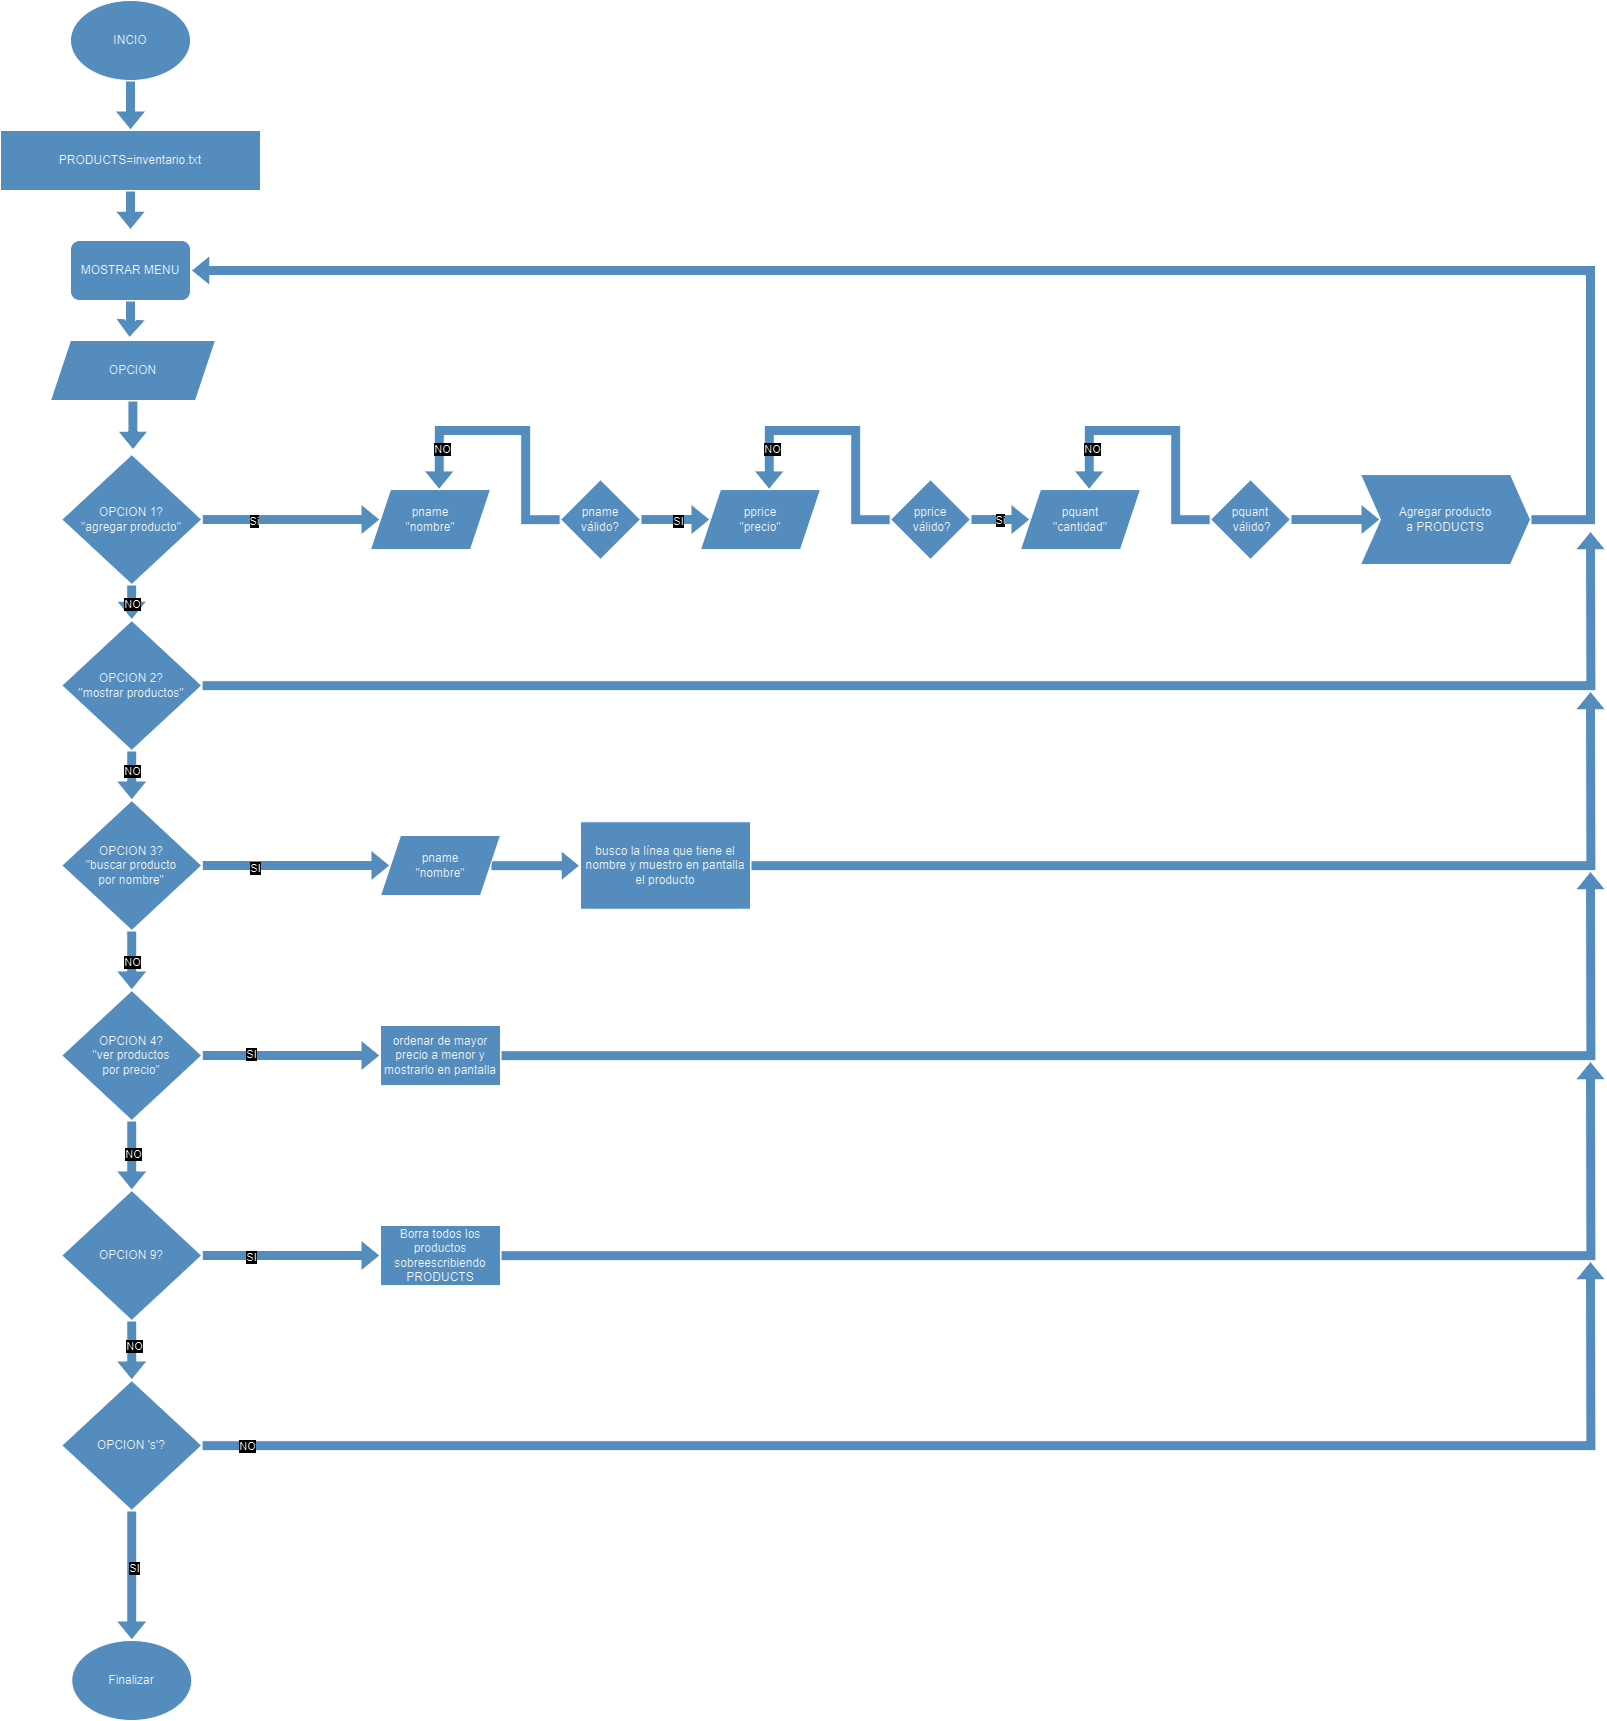
\includegraphics[width=0.43\textwidth]{./diagrama_flujo_tp1.png}
  \caption{Diagrama de flujo del algoritmo}
  \label{img:diag_flujo}
\end{figure}

\section{Código}
Hay algunas partes del código que vale la pena mencionar y explicar en produndidad:
\begin{itemize}
  \item \textbf{search\_product():} en esta función se busca un producto, para lo cual se empleó \textit{grep} con la \textit{flag} de ennumerar lineas (\textbf{-n}), así se puede volver a iterar sobre los productos, y encontrar la línea con todos los datos correspondientes al encontrado.
  \item \textbf{add\_product():} en esta función se agrega un producto, cada dato correspondiente al mismo debe cumplir un cierto formato, por lo que se hacen buclen internos que permiten corroborar que se cumplen las condiciones. Para poder inferir las condiciones se emlea \textit{grep} con las flags que permiten el uso de expresiones regulares.
  \item \textbf{recursión del menu principal:} en vez de emplear un \textit{while} para mostrar el menu princial, se empleó recursión, haciendo que se llame a la función de generar el menu después de cada opción.
  \item \textbf{empleo del less:} en general para mostrar los datos al usuario se hace uso de \textit{less}, facilitando e integrando el uso del programa. 
\end{itemize}

\section{Diagrama de flujo}
El diagrama de flujo se presenta junto a este archivo en diferentes formatos, para la facilidad del lector.

\end{document}
